\section{Start Counter}\label{sec:clas.st}

The start counter, Figs.~\ref{fig:clas.st} and~\ref{fig:clas.stxsection}, is a \abbr{PMT}-instrumented scintillator detector that surrounds the CLAS cryotarget hermetically. It consists of 24 scintillation paddles divided into six sectors matching that of \abbr{CLAS}. Each sector of the start counter is constructed of four independently-instrumented scintillator strips. Timing resolution of the start counter is $\sim$350~ps. The start counter information was used the \g12 triggers~\ref{sec.data.trig.lepton}. More information on the CLAS start counter can be found in \cite{clas.st}.

\begin{figure}[h!]\begin{center}
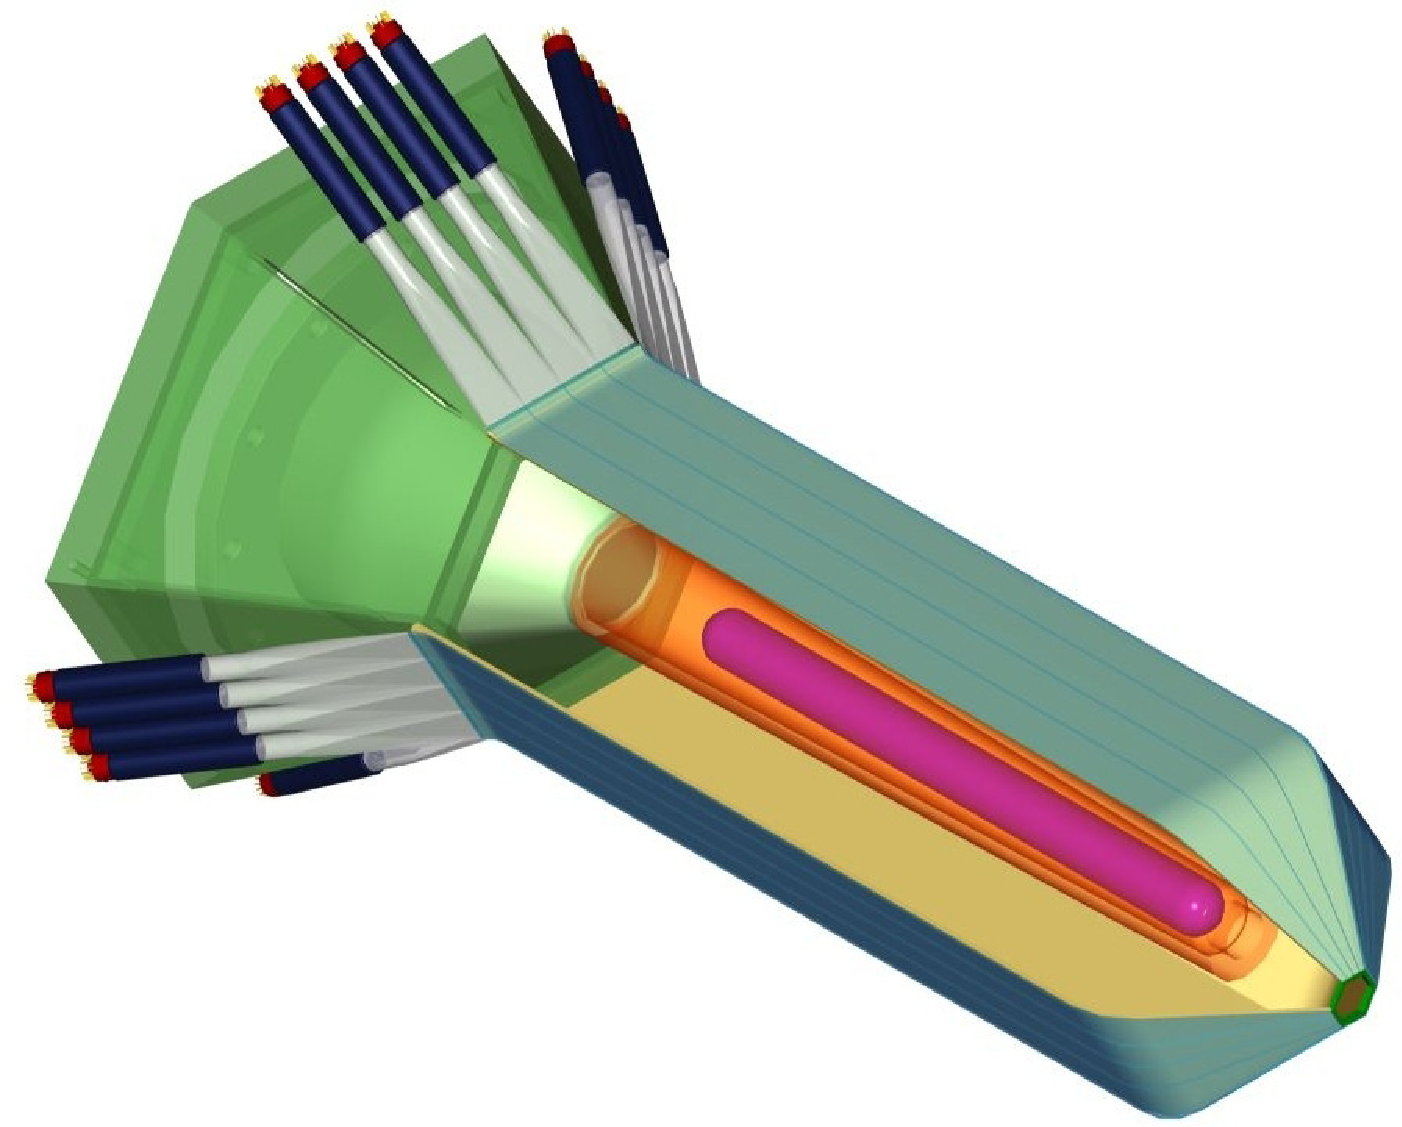
\includegraphics[width=0.8\figwidth,height=\qfigheight]{\grpath/hall-b/start_counter.pdf}
\caption[Schematic of the start counter (\abbr{ST}) with the 40~cm long target cell (purple) at the center]{\label{fig:clas.st}{\coloronline}Schematic of the start counter (\abbr{ST}) with the 40~cm long target cell (purple) at the center. The beam enters from the upper left of the figure.}
\end{center}\end{figure}

\begin{figure}[h!]\begin{center}
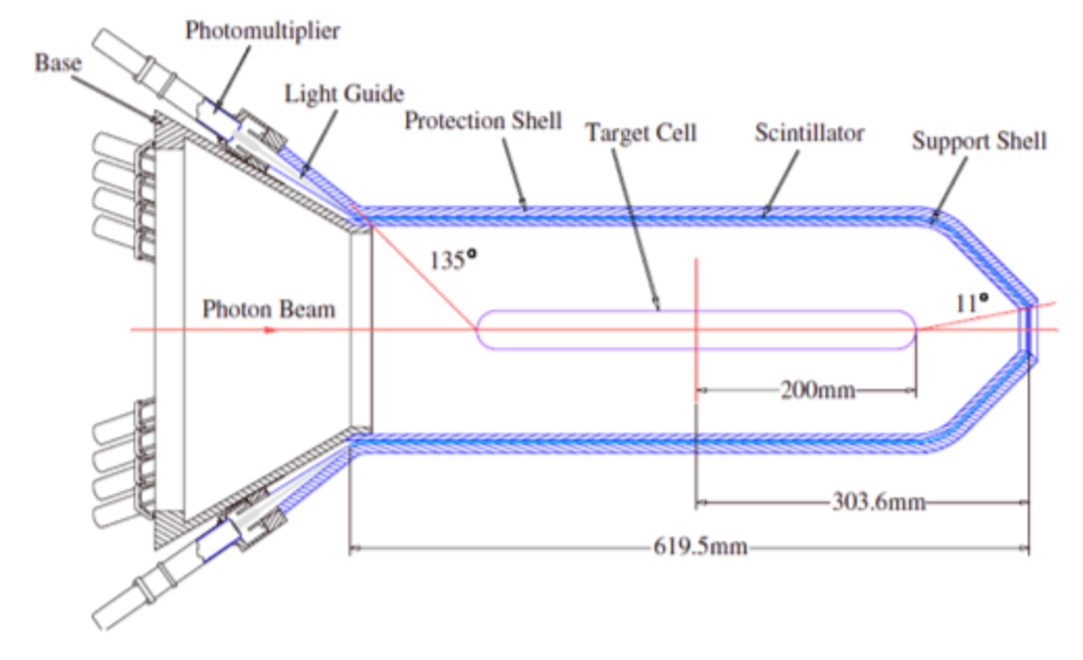
\includegraphics[width=0.8\figwidth,height=\qfigheight]{\grpath/hall-b/start_counter_wtarget.pdf}
\caption[Cross-section view of the start counter illustrating the labeled components and its angular coverage when at the center of \abbr{CLAS}]{\label{fig:clas.stxsection}{\coloronline}Cross-section view of the start counter illustrating the labeled components and its angular coverage when at the center of \abbr{CLAS}.}
\end{center}\end{figure}

\FloatBarrier
%\subsection{Start Counter Efficiency Analysis}\label{sec:clas.st.eff}
%There is an inefficiency of the start counter as seen in Fig.~\ref{fig:classt.ineff}. This inefficiency was measured by using real data events as generated events and passing them through \abbr{CLAS}'s Monete-Carlo package(\abbr{GSIM}\label{abbr:gsim}). More information about this inefficiency will be discussed in Sec.~\ref{sec:analysis.accept.verify}.
%
%%It was observed that 20~\% of the events would fail in simulation, this will be discussed in Sec~\ref{sec:gsim.efficiency}. A portion of the failed events were based upon a failure to reconstruct the required banks for the start counter. This phenomena was investigated from the raw data and found to also be present in the processing of the data from raw to user file in the same manner as seen from Monte-Carlo. The blue-dashed line in Fig.~\ref{fig:classt.ineff} illustrates the start counter inefficiency that is dependent on the events reconstructed vertex. The inefficiency is due to the start counter reconstruction algorithm not being able to link the start counter hit to a track through time-based tracking. This track is not lost due to a reprocess of time-based tracking, linking the track to another particles start counter hit with the same 
%
%%The inefficiency of the start counter is not a mechanical fault but rather the fault of the algorithm used to reconstruct a start counter hit. TO study this raw data events were processed event by event using the program DDD and \abbr{CLAS} event display (\abbr{ced}). Unknown of the cause, it  
%
%
%\begin{figure}[h!]\begin{center}
%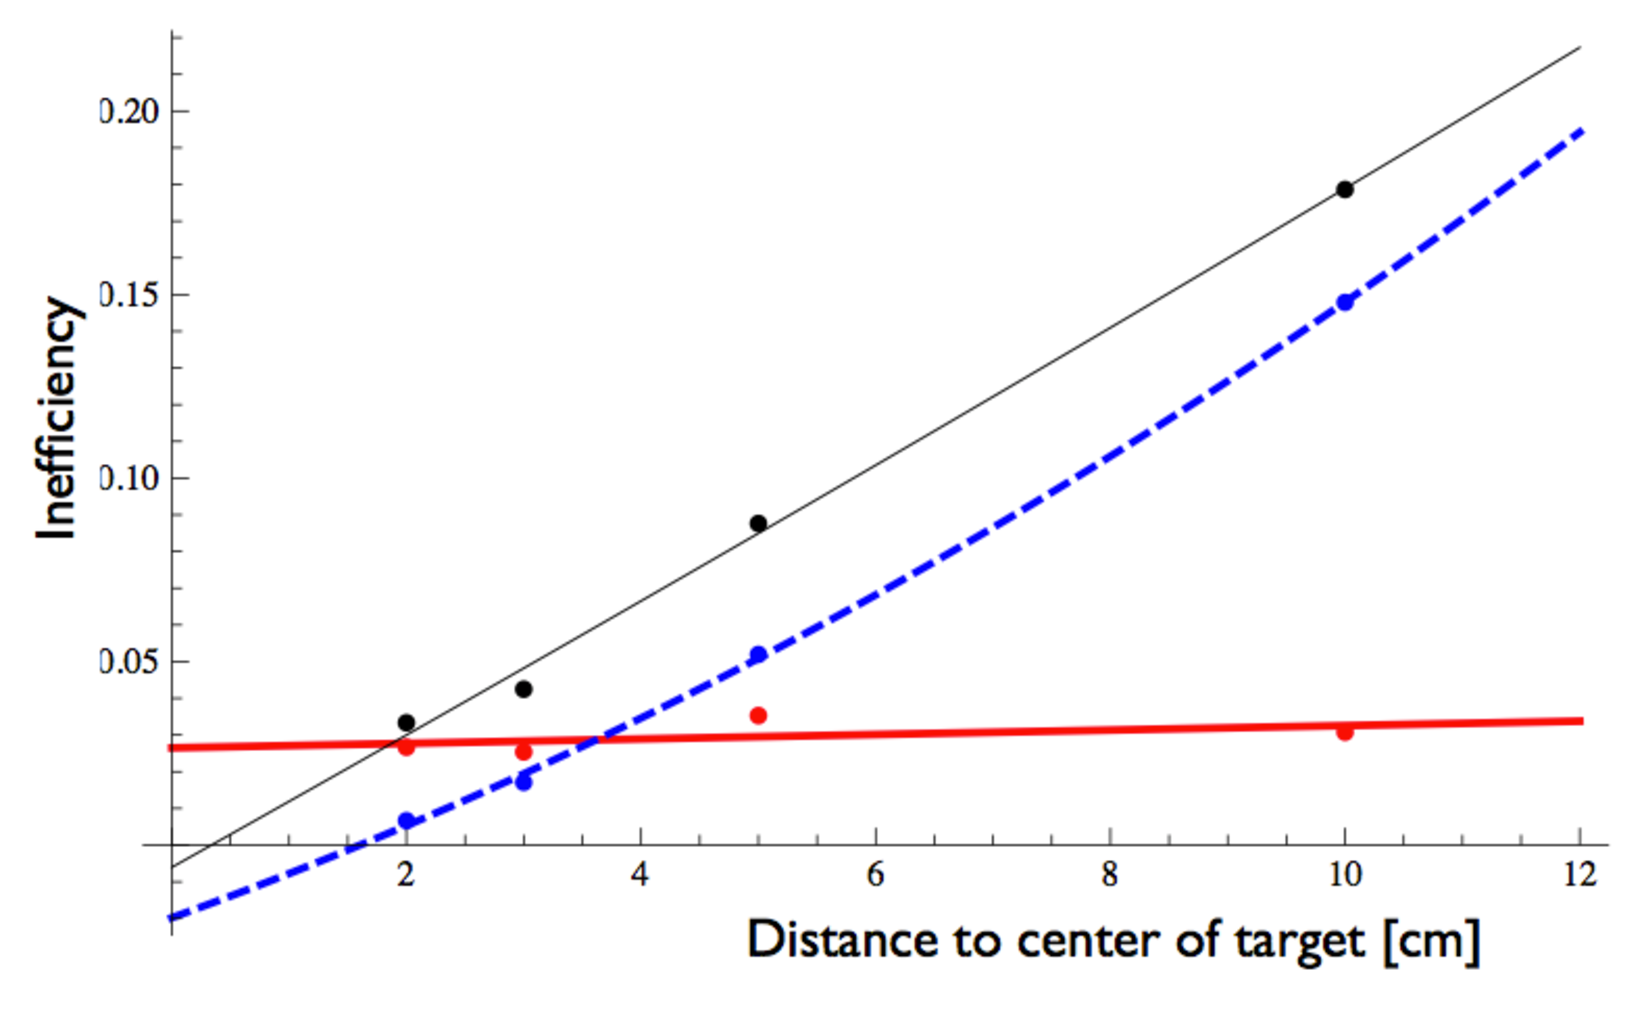
\includegraphics[width=0.8\figwidth,height=0.7\hfigheight]{\grpath/hall-b/st_issue_4_thesis.pdf}
%\caption[Start Counter Inefficiency]{\label{fig:classt.ineff}{\coloronline}Plot showing the inefficiency of the start counter from data events, red-solid line is the inefficiency of reconstruction based solely on hit-based tracking, blue-dashed line is inefficiency of start counter, black-solid is combined. }
%\end{center}\end{figure}
%
%\FloatBarrier